\documentclass[11pt, oneside]{article}   	% use "amsart" instead of "article" for AMSLaTeX format
\usepackage{geometry}                		% See geometry.pdf to learn the layout options. There are lots.
\geometry{letterpaper}                   		% ... or a4paper or a5paper or ... 
%\geometry{landscape}                		% Activate for for rotated page geometry
%\usepackage[parfill]{parskip}    		% Activate to begin paragraphs with an empty line rather than an indent
\usepackage{graphicx}				% Use pdf, png, jpg, or eps� with pdflatex; use eps in DVI mode
								% TeX will automatically convert eps --> pdf in pdflatex		
\usepackage{amssymb}
\usepackage{amsmath}
\usepackage{parskip}
\usepackage{color}

\title{Introduction to surface integrals 2}
%\author{The Author}
%\section{}
% \subsection*{R code}
\date{}							% Activate to display a given date or no date

\graphicspath{{/Users/telliott_admin/Dropbox/Tex/png/}}

% \begin{center} 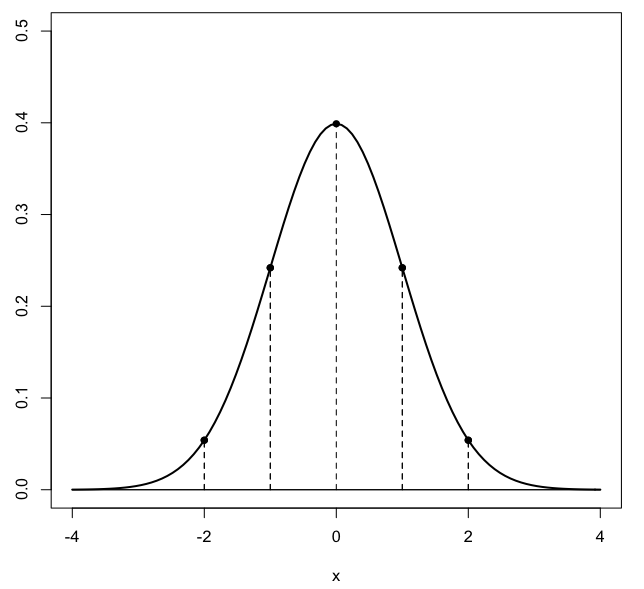
\includegraphics [scale=0.4] {gauss3.png} \end{center}
% \begin{bmatrix} a  &  b \\ c  &  d \end{bmatrix}
% \bigg |_

\begin{document}
\maketitle
\large
%\noindent
The theorem for surface integrals is that the area element is given by
\[ dS = \sqrt{(f_x)^2 + (f_y)^2 + 1} \ \ dx \ dy \]
\[ A(S) = \iint_{D} 1 \ dS =  \iint_{R} \sqrt{(f_x)^2 + (f_y)^2 + 1} \ \ dA \]

In this short write-up, we want to see where this comes from.  Consider a surface formed by 
\[ z = f(x,y) \]
at a point $P=(x_0,y_0)$.  Slice by a plane parallel to the $xz$-axis ($y=y_0=const$).  Consider what happens to $z$ as we move to $x=x_0 + \Delta x$.  Using the linear approximation, the vector along our path is
\[ \mathbf{u} = \ < \Delta x, 0, f_x \Delta x > \ =  < 1,0,f_x> \ \Delta x \]
The vector above is parallel to the surface in the direction where $\Delta y=0$.  Similarly $\mathbf{v}$ is parallel to the surface in the direction where $\Delta x=0$
\[ \mathbf{v} = \ < 0, \Delta y, f_y \Delta y > \ =  < 0,1,f_y>  \ \Delta y \]
and 
\[ \mathbf{n} =  \mathbf{u} \times  \mathbf{v} \]
\[ =  \ <-f_x,-f_y,1> \ \Delta x \ \Delta y \]
\subsection*{dS}
If we consider the relationship between the surface area element $dS$ and the shadow that it casts in the $xy$-plane, $dR$, the "exchange rate" is
\[ \cos \theta \ dS = dR \]

\begin{center} 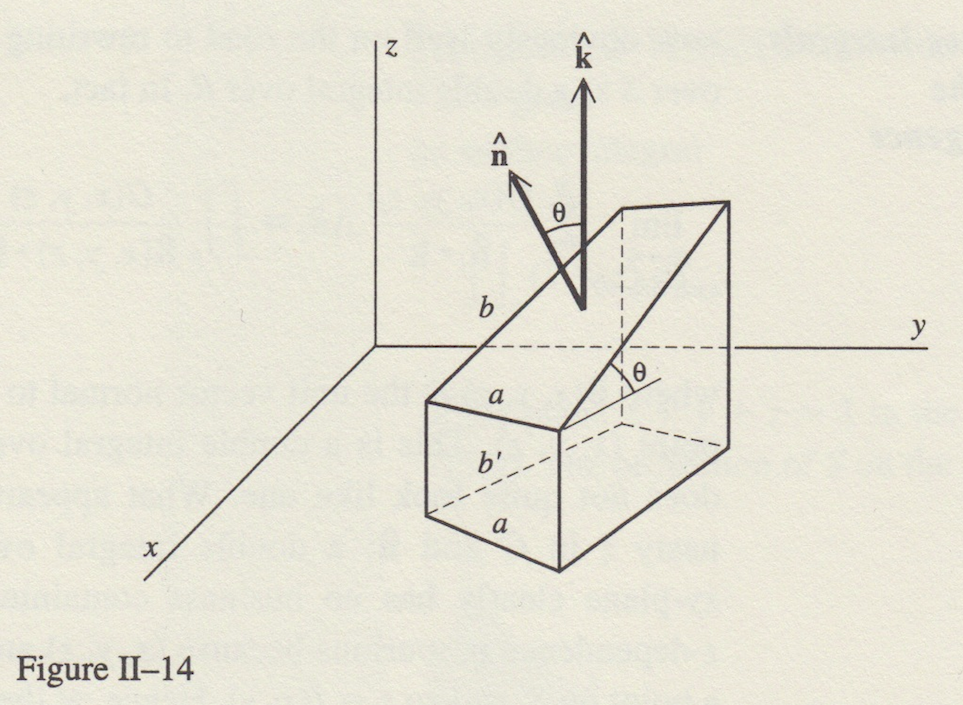
\includegraphics [scale=0.3] {tilt.png} \end{center}

$dR$ is smaller than $dS$ by a factor $\cos \theta$ which is just
\[ \cos \theta =  \hat{\mathbf{n}} \cdot \hat{\mathbf{k}} \]
\[ \hat{\mathbf{n}} \cdot \hat{\mathbf{k}} \ dS = dR \]
\[ dS = \frac{1}{\hat{\mathbf{n}} \cdot \hat{\mathbf{k}}} \ dR \]
What is $\hat{\mathbf{n}}$?  We need to divide $\mathbf{n}$ by $|\mathbf{n}|$.  Compute compute $|\mathbf{n}|$ and set it equal to k
\[ \mathbf{n} =  \ <-f_x,-f_y,1> \ \Delta x \ \Delta y \]
\[ |\mathbf{n}| = k = \sqrt{f_x^2 + f_y^2 + 1} \ \Delta x \ \Delta y  \]
\[ \hat{\mathbf{n}} = \frac{1}{k} \mathbf{n} =  \frac{1}{k}  \ <-f_x,-f_y,1> \]
So
\[ \hat{\mathbf{n}} \cdot \hat{\mathbf{k}} = \frac{1}{k} \]
Finally
\[ dS = k \ dR =  \sqrt{f_x^2 + f_y^2 + 1} \ dR \]
Note then we finally do $\int \mathbf{F} \cdot \hat{\mathbf{n}} \ dS$
this will become
\[ \int \mathbf{F} \cdot  \frac{1}{k}  \ <-f_x,-f_y,1> \ k \ dR =  \int \mathbf{F} \cdot  \ <-f_x,-f_y,1>  \ dR \]  


\end{document}  